% 1-form symmetry defect braiding with a Wilson line in 3+1d.
% The surface operator U(Sigma) (codimension-2, i.e. 2-dimensional) links
% with the Wilson line W_R(C) (1-dimensional), producing a phase exp(2*pi*i*q/N).
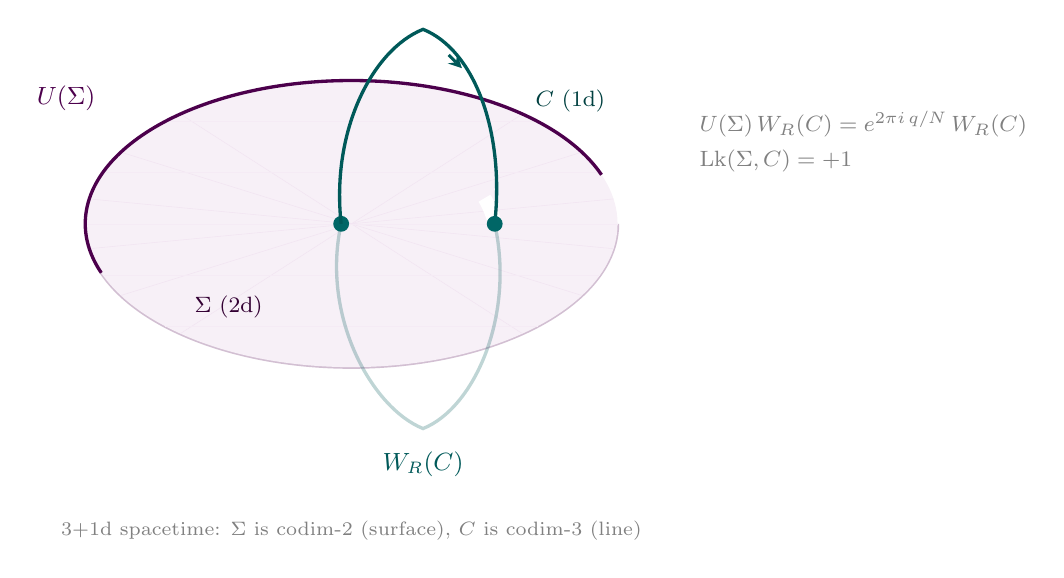
\begin{tikzpicture}[scale=1.3, thick,
    surface color/.style={fill=violet!8, draw=violet!50!black},
    surface edge/.style={very thick, violet!60!black},
    wilson/.style={very thick, teal!70!black},
    faded/.style={opacity=0.25}]

  % === Surface operator U(Sigma): a tilted disk (2d object in 3+1d) ===
  % Drawn as an ellipse with shading to suggest a 2d membrane.

  % Back edge of surface (behind Wilson line)
  \draw[surface edge, faded] (0,0) ++(200:2.6 and 1.4) arc (200:360:2.6 and 1.4);

  % Surface fill
  \fill[fill=violet!6] (0,0) ellipse (2.6 and 1.4);
  % Cross-hatching to emphasize 2d extent
  \foreach \ang in {-50,-30,...,50} {
    \pgfmathsetmacro{\xa}{2.6*cos(\ang)}
    \pgfmathsetmacro{\ya}{1.4*sin(\ang)}
    \pgfmathsetmacro{\xb}{2.6*cos(\ang+180)}
    \pgfmathsetmacro{\yb}{1.4*sin(\ang+180)}
    \draw[violet!10, very thin] (\xa, \ya) -- (\xb, \yb);
  }
  % Horizontal hatching
  \foreach \y in {-1.0,-0.5,...,1.0} {
    \pgfmathsetmacro{\xext}{2.6*sqrt(max(0.001, 1 - (\y/1.4)*(\y/1.4)))}
    \draw[violet!8, very thin] (-\xext, \y) -- (\xext, \y);
  }

  % Front edge of surface
  \draw[surface edge] (0,0) ++(200:2.6 and 1.4) arc (200:180:2.6 and 1.4)
    arc (180:20:2.6 and 1.4);

  % === Wilson line W_R(C): a vertical loop threading through the surface ===
  % Parameterized as an ellipse in the xz-plane, centered at (0.4, 0).
  % "Threading through" means it pierces the surface once going up, once going down.

  % Back arc of Wilson line (below surface)
  \draw[wilson, faded]
    (-0.1, 0.0)
    .. controls (-0.3, -0.9) and (0.2, -1.8) .. (0.7, -2.0)
    .. controls (1.2, -1.8) and (1.6, -0.9) .. (1.4, 0.0);

  % Piercing point (Wilson line emerges from surface)
  \fill[teal!80!black] (-0.1, 0.0) circle (2.2pt);

  % White knockout where Wilson line crosses over surface edge on right
  \draw[white, line width=5pt]
    (1.3, 0.25) .. controls (1.38, 0.12) and (1.4, 0.0) .. (1.4, 0.0);

  % Front arc of Wilson line (above surface)
  \draw[wilson]
    (-0.1, 0.0)
    .. controls (-0.2, 0.9) and (0.2, 1.7) .. (0.7, 1.9)
    .. controls (1.2, 1.7) and (1.5, 0.9) .. (1.4, 0.0);

  % Orientation arrow on Wilson line
  \draw[teal!70!black, ->, >=stealth, line width=1.1pt]
    (0.95, 1.65) -- (1.08, 1.52);

  % Second piercing point (Wilson line re-enters surface)
  \fill[teal!80!black] (1.4, 0.0) circle (2.2pt);

  % === Labels ===
  % Surface label
  \node[violet!60!black, font=\small, anchor=south east] at (-2.4, 1.0)
    {$U(\Sigma)$};
  \node[violet!40!black, font=\footnotesize, anchor=north] at (-1.2, -0.6)
    {$\Sigma$ \textrm{\footnotesize (2d)}};

  % Wilson line label
  \node[teal!70!black, font=\small] at (0.7, -2.35) {$W_R(C)$};
  \node[teal!50!black, font=\footnotesize, anchor=west] at (1.7, 1.2)
    {$C$ \textrm{\footnotesize (1d)}};

  % Linking phase annotation
  \node[font=\footnotesize, gray, anchor=north west, align=left] at (3.3, 1.2)
    {$U(\Sigma)\, W_R(C) = e^{2\pi i \, q/N}\, W_R(C)$\\[3pt]
     \footnotesize $\mathrm{Lk}(\Sigma, C) = +1$};

  % Dimension annotation
  \node[font=\scriptsize, gray, anchor=north] at (0, -2.8)
    {3+1d spacetime: $\Sigma$ is codim-2 (surface), $C$ is codim-3 (line)};

\end{tikzpicture}
